
\begin{figure*}
      \centering
      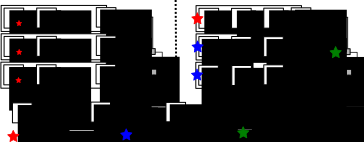
\includegraphics[width=0.95\textwidth]{fig/overview.png}
      %%
      \caption{~\todo{redo diagram to remove memory centric
      organization (it's a pipe dream)}
      Anatomy of a disaggregated rack. On the left a
      traditional rack with processors colocated with their memory
      interconnected by a switch. On the right is a high density
      disaggregated rack with processors separated from their memory
      by a top of rack switch. Stars mark locations for memory access
      serialization. Red denotes traditional processor centric
      serialization~\cite{memc3, cell, sonuma, storm, clover}, blue marks a
      memory centric architecture~\cite{aguilera2019designing}, and
      green marks a switch centric solution similar in spirit to
      proposed middle box solutions~\cite{254120}.
      \label{fig:overview}
      %%
      }
\end{figure*}

\section{Clover}

%%

Clover is designed empirically to maximize read performance to passive
remote memory. It separates key value metadata from the datapath, and
from clients. Clients issue lockless reads to passive memory servers,
and opportunistic writes using RDMA compare and swap (CNS) to keep
remote writes consistent. When writes succeed clients update metadata
severs lazily. If reads or writes fail because clients have stale
metadata they concurrently requests fresh metadata, and traverse
remote memory to obtain the freshest information (a processes known as
pointer chasing). They found this approach to obtain extremely high
throughput with read heavy workloads as updates are rare and clients
enjoy unfettered access to remote memory. In contrast they found that
placing a metadata coordinator in the datapath became a bottleneck at
only a fraction of their achievable throughput.


In the presence of writes however clovers operation throughput
decreases due to contention. When concurrent writes contest the same
data a race occurs in which the fastest writer wins. Write operations
require two messages, a data update (RDMA WRITE) and (RDMA CNS) which
updates old data to point to the new version. During this two RTT
operation any concurrent write to the same key will cause a conflict.
The slower writers will fail, and must retry their write after
searching through remote memory or by getting an update from the
metadata server.  On write heavy workloads these race conditions
happen frequently as illustrated in Figure~\ref{fig:conflicts}, which
leads to a sharp decrease in throughput.

We propose a middle ground between Clover and a centralized approach.
Our insight is that by using data structure specific knowledge, and
caching write locations in network conflicting writes can be resolved
resolved at line rate in the data path.  Using Clover as a platform to
prove our concept we design a middle box algorithm which intercepts
clovers RDMA read and write request, caches a small amount (64 byte
per key) of structural meta data and resolves write conflicts by
adjusting the destination RDMA virtual address of the writes. Our
algorithm is implemented in DPDK, but is designed to have low memory
and computational overhead making it ideal for network devices such as
programmable switches and NICs.


%% The high level pitch about remote memory.
%Far memory projects typically have a remote CPU which is used to
%coordinate access to remote resources (cite all object systems). In a
%disaggregated system there is no remote CPU, therefore the coordination
%of reads and writes to remote locations must be done locally. For
%performance local caches of remote resources can be used to organize
%access to remote resources. For data structures which require
%consistency this creates a problem as stale caches can lead to data
%structure corruption.

\section{Write Conflict Resolution}

%Our system caches metadata for remote data structure on centralized
%networking devices. Our prototype is implemented in DPDK, however our
%algorithm could be implemented on a programmable switch or
%programmable NIC as long as it sees all requests to remote memory. 
%% kinds of devices
%A programmable TOR or our DPDK switch (which behaves as one) is ideal
%for rack scale disaggregated structures that potentially span multiple
%memory servers, while a programmable NIC implementation would be
%limited limited to the memory server it is attached to. 

%%Technique example
The purpose of our technique is to resolve write conflicts to remote
memory. As an illustrative example of a conflict consider a linked
list implemented as a remote memory data structure with a single
operation, \textit{appendTail}. This operation ensures that the next
write to the data structure writes to the tail of the linked list.
This operation requires two steps.  First a writer sends and RDMA
write to remote memory which writes the new data value for the tail to
a scratch space. After the data is written a second operations
consisting of an RDMA compare and swap (CNS) is issued to the old tail
which replaces it's NULL next pointer with the address of the prior
write.

This operation succeeds every time in the single threaded case as the
tail of the linked list is never moved by another process. Consider
instead the multi-threaded case in which two writers both attempt to
execute \textit{appendTail} concurrently. Both issue their first write
to remote memory successfully and then attempt to run an RDMA CNS on
the tail of the old list. This results in a race condition where the
first process to write succeeds, and the other will fail. The process
which executes the CNS second fails because rather than finding a tail
with a next value of NULL, it finds the now penultimate member of the
linked list which now points to the value issued by the process which
won the race. 

The process which lost the race now needs to engage in \textit{Pointer
chasing} to find the new tail. It must iterative issue reads of the
linked list, step by step until it finds the location of the new tail.
At which point it can reissue a CNS to make the new tail point to it's
value. The reissued CNS is also subject to the same race condition as
many writers may be execution \textit{appendTail}. This reconciliation
algorithm of pointer chasing must be run each time a conflict occurs.
For highly contested structures, the number of retries can grow
quickly, leading to large and unpredictable tail latencies.

In the case of clover this exact scenario occurs when key are write
contested. Their experiments with a zipf distribution on their keys
sees a 5x reduction in throughput at 50\% writes.

%% What do we actually do
If a central arbiter where to observer the writes to this linked list
it would notice that the second CNS does not need to fail, it simply
needs to be redirected to point at the new tail of the list. 
%%
Our observation is that such a coordinator can be implemented in
network can significantly improve throughput. Using data structure
specific information the coordinator can cache recent writes, and
steer concurrent ones to locations which will result in successful
operations and maintain the correctness of the remote data structure.

In Clover each key value pair has versioning in the form of a linked
list which operates identically to the \textit{appendTail} operation
described above. We cache the tail of the linked list for each key in
clovers key value store. This results in an \textit{O(n)} overhead
where n is the number of keys. In our case for a key value store
consisting of 10k keys we need to store a key mapping and value for
each (both 64 bits) resulting in a total in network storage of 80KB.
Note that this O(n) overhead is only a small fraction of clovers
metadata which contains all key versions of the linked list. However
only the tail of the list is required to resolve write conflicts.

\textbf{Modifying RDMA in flight:} Interposing on an RDMA protocol is
non trivial. One solution (evaluated in as Clover
pDPM-central~\cite{clover}) would be to use an RDMA enabled middlebox
to setup connections between the clients and the memory servers which
would reissue RDMA request to the consistent locations. This solution
is impossible for a switch as it lacks the capabilities and resources
to establish RDMA connections. Further it has been demonstrated to be
a performance bottleneck. Our algorithm interposes on RDMA requests
transparently without storing any explicit RDMA state, or establishing
connections.

When RDMA write requests are issued our algorithm stores the locations
of the virtual addresses of the writes for each client thread. These
writes are marked as \textit{outstanding}. Outstanding writes are
writes which have been made to remote memory, but which have not yet
been made consistent in Clover. Outstanding writes are not yet
connected to Clovers key linked lists and therefore cannot be read by
other clients. Following an outstanding write clients will issue an
RDMA CNS which points the tail of the last committed write to the last
outstanding write the client issued, making it the new tail of the
list. Our algorithm detects the existence of a conflict when there is
more than one outstanding write for a given key. In addition to
tracking outstanding writes per client, our algorithm tracks the last
CNS issued to each key. This CNS marks the true tail of a keys linked
list. When a CNS for an outstanding write is seen, and the virtual
address of it's CNS points to an old tail, it's virtual address is
modified in flight (without the knowledge of the issuing client) to
point to the true tail of the list. The cached latest version of the
key is then updated to point to the address the CNS was directed to.
Clover clients learn the updated locations using their default read
algorithm.

RDMA packets are not intended to be modified in flight, and care must
be taken no to corrupt them. RDMA invariant CRCs (ICRC) are calculated
at the time of sending and are designed to ensure the integrity of the
payload. When we modify CNS packets their ICRC must be recalculated or
the packet will be rejected by the receiving NIC. FPGA implementations
of RDMA ICRC have been built in the past~\cite{Mansour_2019}, the
required CRC calculation is identical to ethernet CRC, with the
requirement of additional header injection and field masking. Our DPDK
solution uses zlibs crc32 for the calculation. We believe that this
algorithm can also be implemented efficiently on a programmable
switch.

\section{Evaluation}

Our experimental setup consists of 4 machines each with two sockets
equipped Intel Xeon E5-2640 CPU's and 265GB of main memory evenly
spread across two NUMA domains. Each machine has a Mellanox ConnectX-5
100Gbps NIC installed in a 16x PCIe slot. Each server is
interconnected via a 100Gbps Mellanox Onyx Switch. We designate a
single server to run as both the memory server (MS) and as the meta
data server (DN). Two machines are configured as clients, and a single
machine acts as a programmable switch.

All clover servers are configured using default routing settings.
Clients are configured to send directly to metadata and data servers.
We install OpenFlow rules on our Mellanox Onyx switch to redirect all
traffic to our DPDK packet switch.

\subsection{Conflict Resolution}

We test the performance gains of resolving write conflicts using our
middlebox solution. Clover clients are configured to run a YCSB-A
benchmark, 50\% read, 50\% write for 1 million requests. Request for
keys are distributed based on a zipf distribution generated with an
\textit{s} value of 0.75.\todo{show exactly what this means}. In each
experiment the number of client threads is increased which in turn
increases the load on the system. Clover request are blocking, and
thus the throughput is a factor of both the request latency and the
number of client threads. Figure~\ref{fig:throughput} shows the
performance gains by resolving write conflicts in flight.

As the number of clients increases so to does the probability that two
client threads will make concurrent writes to the same key. The number
of conflicts resolved in flight directly correlates to throughput
improvements as each successful request reduces the multiple round
trips necessary to resolve write conflicts. Our current implementation
provides a 1.42x throughput improvement at 64 client threads.

Our current experiments are limited by the scale of our experimental
setup, i.e more client machines can produce higher throughputs.
\todo{This is the speculation part we should cut}. 
The number of in flight conflicts is also effected by the zipf
distribution. We use a zipf of 0.75, however a zipf of 1.0 would
result in a distribution skewed towards fewer keys, which in turn
would result in higher conflicts. We found that Clovers current design
leads to high contention on ConnectX-5 NIC's as the number of RDMA
compare and swaps to the same memory region across different queue
pairs increases~\cite{design-guidelines}. In future work we plan to
both scale up the number of our client threads. Additionally our
design reduces the need for expensive compare and swap operations as
all cached keys have no conflicts. Our future implementations will
seek to reduce or eliminate CNS and replace them with low overhead
RDMA writes.

\begin{figure}
    \includegraphics[width=0.45\textwidth]{fig/throughput.pdf}
    \caption{Default Clover throughput vs Clover with write conflict
    detection and correction turned on.}
    \label{fig:throughput}
\end{figure}

\subsection{Memory Consumption}

Resources on networking hardware is scarce. High end SoC SmartNIC's
have just a few GB of RAM, and programmable switches have only MB's of
SRAM. Moreover the use of this memory is not free. Using memory for
any purpose other than buffer packets has a direct performance cost as
the number of packets which can be successfully buffered drops. Our
design takes the preciousness of memory in network into account. The
metadata we cache in network in the minimal necessary to resolve write
conflicts. While Clover's meta data consists of many MB of garbage
collection and version data we only cache the virtual address of the
last write per key. In addition we track the last key written per
client thread. Clients are not explicitly known to our middlebox and
are identified at runtime by their QP. Tracking clients in this way is
necessary to detect write conflicts in clover. This overhead could be
eliminated by explicitly adding key information to CNS requests.

Figure~\ref{fig:memory} Shows the memory overhead as a function of
keys. Note that 100K keys can be supported using 7\% of the available
memory on a Barefoot Tofino programmable switch (22MB).

\begin{figure}
    \includegraphics[width=0.45\textwidth]{fig/memory.pdf}
    \caption{Cost of caching metadata in network vs keyspace size.}
    \label{fig:memory}
\end{figure}

\subsection{Caching top \textit{N} keys} 
%%
Hot keys which are written frequently are the most likely to
contribute to conflict. Caching only hot keys results in relatively
large performance gains while requiring only a small portion of the
memory required to cache the entire keyspace. We test the effect of
caching only hot keys by restricting our in network cache to track and
resolve conflicts on only the top \textit{N} keys. In this experiment
RDMA requests for keys which are not caches pass through our middlebox
without modification, conflicts are resolved using Clovers
reconciliation protocol. We ran our experiment with 64 client threads,
with a total keyspace size of 1024 keys. Figure~\ref{fig:cache} shows
the relative throughput gains from caching the top N keys. The request
distribution is zipf(0.75), therefore the vast majority of conflicts
occur on the top 8 keys. The in network memory requirement for 8 keys
is 128 Bytes, which results in 1.3x throughput improvement.

\begin{figure}
    \includegraphics[width=0.45\textwidth]{fig/cache.pdf}
    \caption{Performance as a function of keys cached. Caching a few
    of the top n keys provides the greatest marginal throughput
    benefits.}
    \label{fig:cache}
\end{figure}

\section{Future Work}

